\let\negmedspace\undefined
\let\negthickspace\undefined
\documentclass[journal]{IEEEtran}
\usepackage[a5paper, margin=10mm, onecolumn]{geometry}
%\usepackage{lmodern} % Ensure lmodern is loaded for pdflatex
\usepackage{tfrupee} % Include tfrupee package

\setlength{\headheight}{1cm} % Set the height of the header box
\setlength{\headsep}{0mm}     % Set the distance between the header box and the top of the text

\usepackage{gvv-book}
\usepackage{gvv}
\usepackage{cite}
\usepackage{amsmath,amssymb,amsfonts,amsthm}
\usepackage{algorithmic}
\usepackage{graphicx}
\usepackage{textcomp}
\usepackage{xcolor}
\usepackage{txfonts}
\usepackage{listings}
\usepackage{enumitem}
\usepackage{mathtools}
\usepackage{gensymb}
\usepackage{comment}
\usepackage[breaklinks=true]{hyperref}
\usepackage{tkz-euclide} 
\usepackage{listings}
% \usepackage{gvv}                                        
\def\inputGnumericTable{}                   
\usepackage[latin1]{inputenc}                                
\usepackage{color}                                            
\usepackage{array}                                     
\usepackage{longtable}                                       
\usepackage{calc}                                     
\usepackage{multirow}                                         
\usepackage{hhline}                                            
\usepackage{ifthen}                                           
\usepackage{lscape}
\begin{document}

\bibliographystyle{IEEEtran}

\title{5.5.1}
\author{EE25BTECH11049 - Sai Krishna Bakki}
\maketitle

\subsection*{Question: } 
If $\vec{A}=\myvec{5&-1&4\\2&3&5\\5&-2&6}$, find $\vec{A}^{-1}$ and use it to solve the following system of equations
\begin{align*}
    5x-y+4z=5\\
    2x+3y+5z=2\\
    5x-2y+6z=-1
\end{align*}

\textbf{Solution}:
    \begin{align}
        \augvec{3}{3}{5&-1&4& 1& 0&0\\ 2&3&5& 0& 1&0\\5&-2&6& 0& 0&1}
        &\xleftrightarrow{\,R_3 \gets R_3 - R_1}
        \augvec{3}{3}{5&-1&4& 1& 0&0\\ 2&3&5& 0& 1&0\\0&-1&2& -1& 0&1} \end{align}
        \begin{align}
        &\xleftrightarrow[\,R_2 \gets R_2 + 3R_3]{\,R_1 \gets R_1 - R_3}
        \augvec{3}{3}{5&0&2& 2& 0&-1\\ 2&0&11& -3& 1&3\\0&-1&2& -1& 0&1}\end{align}
        \begin{align}
        &\xleftrightarrow{\,R_3 \gets -R_3}
        \augvec{3}{3}{5&0&2& 2& 0&-1\\ 2&0&11& -3& 1&3\\0&1&-2& 1& 0&-1} \end{align}
        \begin{align}
        &\xleftrightarrow{\,R_2 \leftrightarrow R_3}
        \augvec{3}{3}{5&0&2& 2& 0&-1\\ 0&1&-2& 1& 0&-1\\2&0&11& -3& 1&3} \end{align}
        \begin{align}
        &\xleftrightarrow{\,R_1 \gets \frac{1}{5}R_1}
        \augvec{3}{3}{1&0&2/5& 2/5& 0&-1/5\\ 0&1&-2& 1& 0&-1\\2&0&11& -3& 1&3} \end{align}
        \begin{align}
        &\xleftrightarrow{\,R_3 \gets R_3 - 2R_1}
        \augvec{3}{3}{1&0&2/5& 2/5& 0&-1/5\\ 0&1&-2& 1& 0&-1\\0&0&51/5& -19/5& 1&17/5} \end{align}
        \begin{align}
        &\xleftrightarrow{\,R_3 \gets \frac{5}{51}R_3}
        \augvec{3}{3}{1&0&2/5& 2/5& 0&-1/5\\ 0&1&-2& 1& 0&-1\\0&0&1& -19/51& 5/51&17/51} \end{align}
        \begin{align}
        &\xleftrightarrow[\,R_2 \gets R_2 + 2R_3]{\,R_1 \gets R_1 - \frac{2}{5}R_3}
        \augvec{3}{3}{1 & 0 & 0 & 28/51 & -2/51 & -17/51 \\ 0 & 1 & 0 & 13/51 & 10/51 & -17/51 \\ 0 & 0 & 1 & -19/51 & 5/51 & 17/51}
    \end{align}
    \begin{align}
        \therefore \vec{A}^{-1} = \myvec{ 28/51 & -2/51 & -17/51 \\ 13/51 & 10/51 & -17/51 \\ -19/51 & 5/51 & 17/51 }
    \end{align}
Now, Finding system of equations
\begin{align}
    \vec{A}\vec{X}=\vec{C}
\end{align}
where $\vec{C}=\myvec{5\\2\\-1}$ and $\vec{X}=\myvec{x\\y\\z}$
\begin{align}
    \vec{X}=\vec{A}^{-1}\vec{C}\\
    \vec{X}=\myvec{ 28/51 & -2/51 & -17/51 \\ 13/51 & 10/51 & -17/51 \\ -19/51 & 5/51 & 17/51 }\myvec{5\\2\\-1}\\
    \therefore \vec{X}=\myvec{3\\2\\-2}
\end{align}
\newpage
\begin{figure}
    \centering
    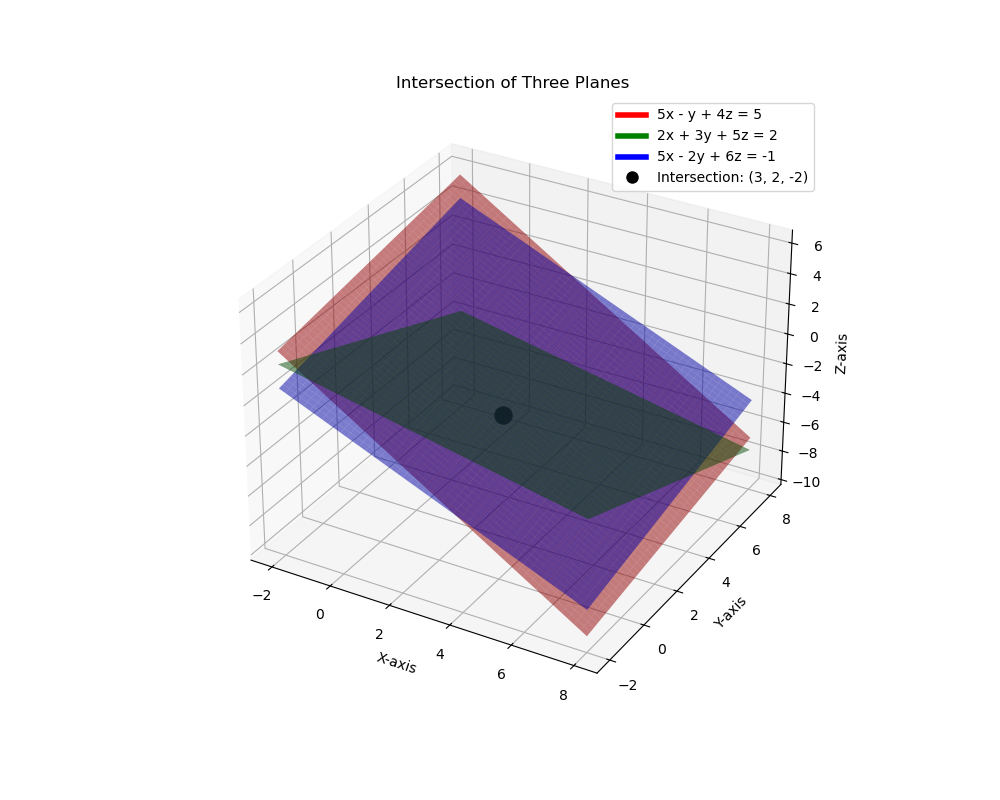
\includegraphics[width=1.2\columnwidth]{figs/Figure_1.png}
    \label{fig:placeholder}
    \caption{}
\end{figure}

\end{document}
